\documentclass[a4paper, 14pt]{extarticle}

% Поля
%--------------------------------------
\usepackage{geometry}
\geometry{a4paper,tmargin=2cm,bmargin=2cm,lmargin=3cm,rmargin=1cm}
%--------------------------------------


%Russian-specific packages
%--------------------------------------
\usepackage[T2A]{fontenc}
\usepackage[utf8]{inputenc} 
\usepackage[english, main=russian]{babel}
%--------------------------------------

\usepackage{textcomp}

% Красная строка
%--------------------------------------
\usepackage{indentfirst}               
%--------------------------------------             


%Graphics
%--------------------------------------
\usepackage{graphicx}
\graphicspath{ {./images/} }
\usepackage{wrapfig}
%--------------------------------------

% Полуторный интервал
%--------------------------------------
\linespread{1.3}                    
%--------------------------------------

%Выравнивание и переносы
%--------------------------------------
% Избавляемся от переполнений
\sloppy
% Запрещаем разрыв страницы после первой строки абзаца
\clubpenalty=10000
% Запрещаем разрыв страницы после последней строки абзаца
\widowpenalty=10000
%--------------------------------------

%Списки
\usepackage{enumitem}

%Подписи
\usepackage{caption} 

\newenvironment{longlisting}{\captionsetup{type=listing}}{}

%Гиперссылки
\usepackage{hyperref}

\hypersetup{
  colorlinks=true,
  unicode=true,
}

%Рисунки
%--------------------------------------
\DeclareCaptionLabelSeparator*{emdash}{~--- }
\captionsetup[figure]{labelsep=emdash,font=onehalfspacing,position=bottom}
%--------------------------------------

\usepackage{tempora}

%Листинги
%--------------------------------------
\usepackage{minted}

\renewcommand\listingscaption{Листинг}
\setminted[cpp]{
  frame=single,
  fontsize=\small,
  linenos,
  xleftmargin=1.5em,
}
%--------------------------------------

%%% Математические пакеты %%%
%--------------------------------------
\usepackage{amsthm,amsfonts,amsmath,amssymb,amscd}  % Математические дополнения от AMS
\usepackage{mathtools}                              % Добавляет окружение multlined
\usepackage[perpage]{footmisc}
%--------------------------------------

%--------------------------------------
%			НАЧАЛО ДОКУМЕНТА
%--------------------------------------

\begin{document}

%--------------------------------------
%			ТИТУЛЬНЫЙ ЛИСТ
%--------------------------------------
\begin{titlepage}
\thispagestyle{empty}
\newpage


%Шапка титульного листа
%--------------------------------------
\vspace*{-60pt}
\hspace{-65pt}
\begin{minipage}{0.3\textwidth}
\hspace*{-20pt}\centering

\includegraphics[width=\textwidth]{emblem}
\end{minipage}
\begin{minipage}{0.67\textwidth}\small \textbf{
\vspace*{-0.7ex}
\hspace*{-6pt}\centerline{Министерство науки и высшего образования Российской Федерации}
\vspace*{-0.7ex}
\centerline{Федеральное государственное бюджетное образовательное учреждение }
\vspace*{-0.7ex}
\centerline{высшего образования}
\vspace*{-0.7ex}
\centerline{<<Московский государственный технический университет}
\vspace*{-0.7ex}
\centerline{имени Н.Э. Баумана}
\vspace*{-0.7ex}
\centerline{(национальный исследовательский университет)>>}
\vspace*{-0.7ex}
\centerline{(МГТУ им. Н.Э. Баумана)}}
\end{minipage}
%--------------------------------------

%Полосы
%--------------------------------------
\vspace{-25pt}
\hspace{-35pt}\rule{\textwidth}{2.3pt}

\vspace*{-20.3pt}
\hspace{-35pt}\rule{\textwidth}{0.4pt}
%--------------------------------------

\vspace{1.5ex}
\hspace{-35pt} \noindent \small ФАКУЛЬТЕТ\hspace{80pt} <<Информатика и системы управления>>

\vspace*{-16pt}
\hspace{47pt}\rule{0.83\textwidth}{0.4pt}

\vspace{0.5ex}
\hspace{-35pt} \noindent \small КАФЕДРА\hspace{50pt} <<Теоретическая информатика и компьютерные технологии>>

\vspace*{-16pt}
\hspace{30pt}\rule{0.866\textwidth}{0.4pt}
  
\vspace{11em}

\begin{center}
\Large {\bf Домашняя работа № 1} \\ 
\large {\bf по курсу <<Теория искусственных нейронных сетей>>} \\
\large <<Реализация однослойного персептрона>> 
\end{center}\normalsize

\vspace{8em}


\begin{flushright}
  {Студент группы ИУ9-71Б Афанасьев И. \hspace*{15pt}\\ 
  \vspace{2ex}
  Преподаватель Каганов Ю. Т.\hspace*{15pt}}
\end{flushright}

\bigskip

\vfill
 

\begin{center}
\textsl{Москва 2024}
\end{center}
\end{titlepage}
%--------------------------------------
%		КОНЕЦ ТИТУЛЬНОГО ЛИСТА
%--------------------------------------

\renewcommand{\ttdefault}{pcr}

\setlength{\tabcolsep}{3pt}
\newpage
\setcounter{page}{2}

\section{Цель работы}

\begin{enumerate}
  \item Реализовать на языке высокого уровня однослойный персептрон и проверить его работоспособность на примере
    искусственных данных типа цифр от 0 до 9 и букв русского алфавита. Размер поля 5$\times$4. 
  \item Исследовать работу персептрона на основе использования различных функций активации. (Линейной, сигмоиды,
    гиперболического тангенса, ReLu).
\end{enumerate}

\section{Постановка задачи}

Основной поставленной задачей является разработка каркаса для обучения \textit{многослойных} персептронов --- это сделано для возможности
переиспользования программного кода в последующих домашних заданиях. Реализованный персептрон должен поддерживать произвольное число скрытых слоёв,
параметризацию различными функциями активации и ошибки. Персептрон должен обучаться методом стохастического градиентного спуска с применением метода
обратного распространения ошибки для вычисления градиентов.

\section{Реализация}

Код программы написан на языке C++. Для выполнения матричных операций используется библиотека
\href{https://eigen.tuxfamily.org/index.php?title=Main_Page}{Eigen}.

В листинге \ref{lst:activation_function.h} приводится реализация функций активации: линейной, ReLU, Leaky ReLU, сигмоиды, гиперболического
тангенса и Softmax.

В листинге \ref{lst:cost_function.h} приводится реализация функций ошибки: MSE, кросс-энтропии и дивергенции Кульбака-Лейблера.

В листингах \ref{lst:perceptron.h} и \ref{lst:perceptron.cc} приводится реализация многослойного персептрона, его обучения методом стохастического
градиентного спуска (с mini-batch оптимизацией) с вычислением градиентов методом обратного распространения ошибки, а также фиксирования показателей
ошибки и точности персепторна на тестовых данных для каждой эпохи.

В листингах \ref{lst:data_supplier.h}, \ref{lst:data_supplier.cc}, \ref{lst:util.h} приводится програмнный код генерации данных для обучения,
валидации и тестирования. Задаётся по 10 образцов цифр и букв русского алфавита, для каждого из которых порождается $2^4 = 16$ модификаций. 
Всего сгенерированных данных --- $20 \cdot 16 = 320$, и они равномерно распределяются между данными для обучения, валидации и тестирования в соотношении
$50\%$, $20\%$ и $30\%$ соответственно.

В листинге \ref{lst:main.cc} приводится \texttt{main}-файл с различными конфигурациями однослойного персептрона.

\begin{longlisting}
  \caption{Файл \texttt{activation\_function.h}}
  \inputminted{cpp}{../src/activation_function.h}
  \label{lst:activation_function.h}
\end{longlisting}

\begin{longlisting}
  \caption{Файл \texttt{cost\_function.h}}
  \inputminted{cpp}{../src/cost_function.h}
  \label{lst:cost_function.h}
\end{longlisting}

\begin{longlisting}
  \caption{Файл \texttt{perceptron.h}}
  \inputminted{cpp}{../src/perceptron.h}
  \label{lst:perceptron.h}
\end{longlisting}

\begin{longlisting}
  \caption{Файл \texttt{perceptron.cc}}
  \inputminted{cpp}{../src/perceptron.cc}
  \label{lst:perceptron.cc}
\end{longlisting}

\begin{longlisting}
  \caption{Файл \texttt{data\_supplier.h}}
  \inputminted{cpp}{../src/data_supplier.h}
  \label{lst:data_supplier.h}
\end{longlisting}

\begin{longlisting}
  \caption{Файл \texttt{data\_supplier.cc}}
  \inputminted{cpp}{../src/data_supplier.cc}
  \label{lst:data_supplier.cc}
\end{longlisting}

\begin{longlisting}
  \caption{Файл \texttt{util.h}}
  \inputminted{cpp}{../src/util.h}
  \label{lst:util.h}
\end{longlisting}

\begin{longlisting}
  \caption{Файл \texttt{main.cc}}
  \inputminted{cpp}{../src/main.cc}
  \label{lst:main.cc}
\end{longlisting}

\section{Результаты экспериментов}

При проведении экспериментов некоторые гиперпараметры были фиксированными: количество эпох --- $200$, размер пакета данных (mini-batch),
использующегося при обучении, --- $10$. Коэффициент обучения (learning rate) подбирался индивидуально для каждой конфигурации персептрона.

Количество данных для обучения составляет $160$, валидационных данных --- $60$, тестовых данных --- $100$. Вместе с обозначенными в условии
функциями активации (линейная, ReLU, сигмоида, гиперболический тангенс) используется функция ошибки MSE.

\subsection{Линейная функция активации}

Линейную функцию активации нельзя использовать с алгоритмом обратного распространения ошибки, поскольку её производная --- константа и не 
зависит от входных данных. Результат в этом случае получается бессмысленным.

\subsection{Функция ReLU}

Коэффициент обучения --- $0.1$.

На рисунке \ref{fig:relu_mse_cost} изображено изменение функции ошибки за период обучения персептрона. Здесь и далее
график синей функции соответствует данным для обучения, график оранжевой функции --- тестовым данным. В результате, ошибка на данных
для обучения составляет $0.400494$, ошибка на тестовых данных --- $0.40741$.

\begin{figure}[!htb]
  \centering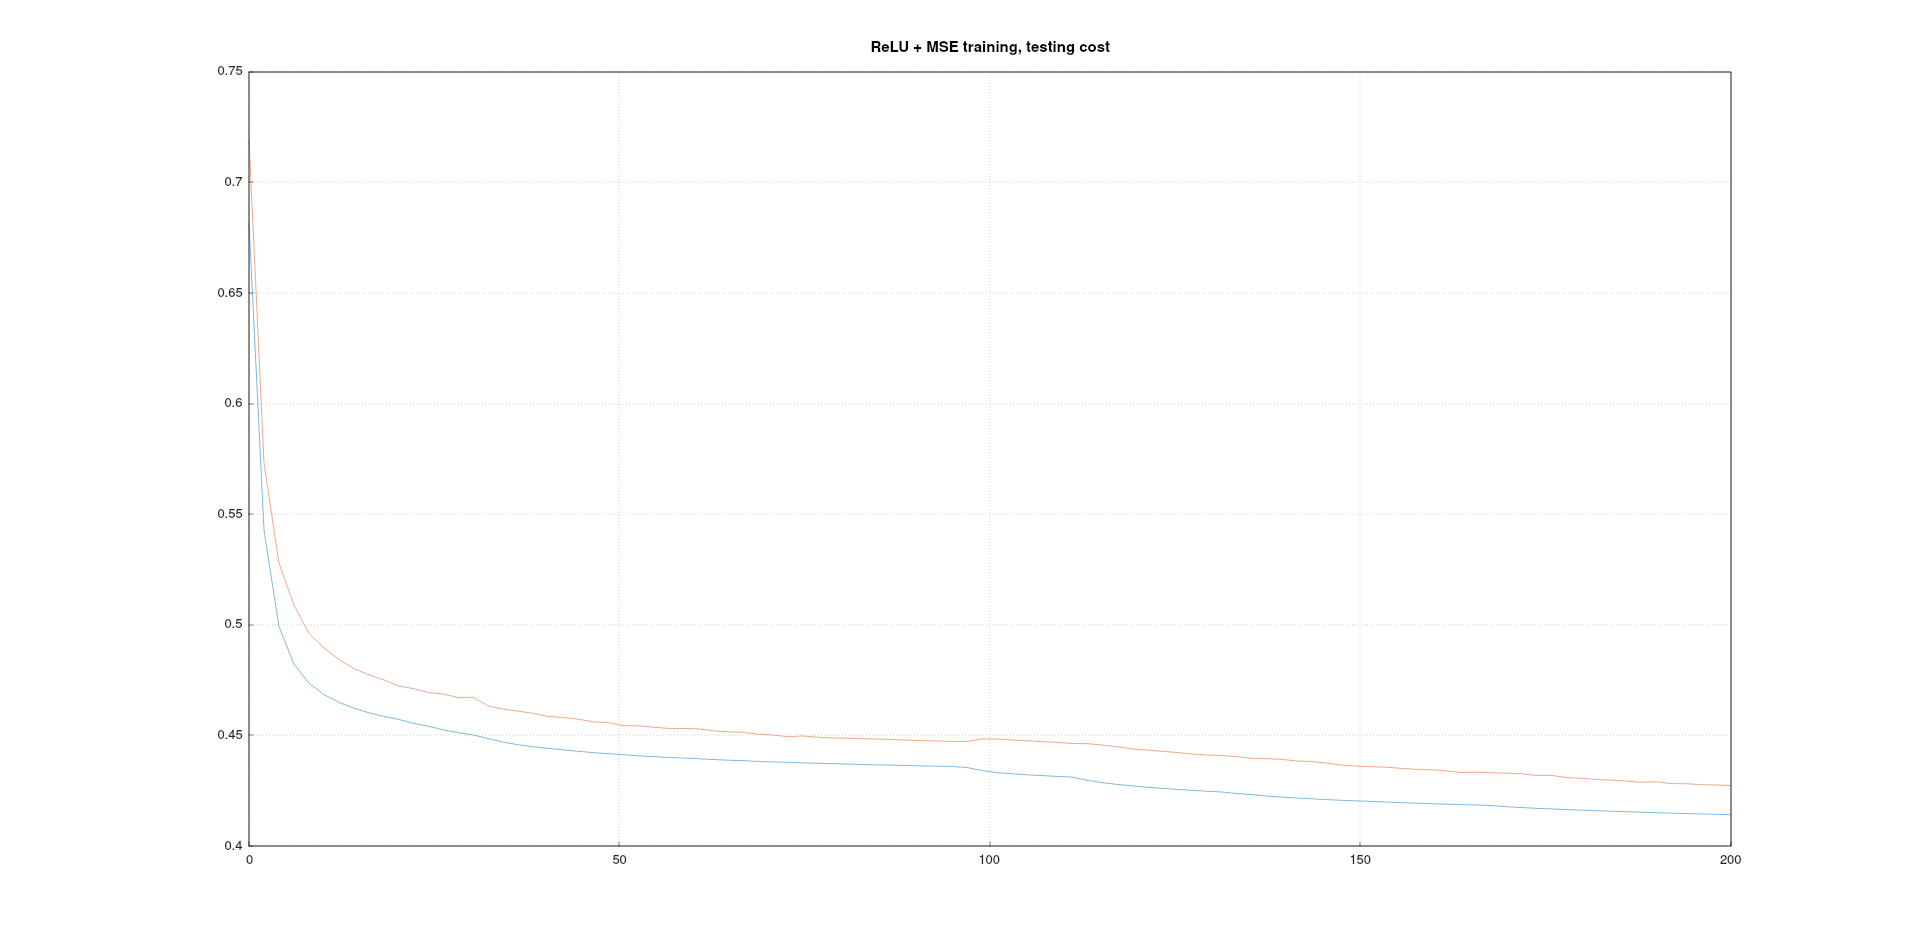
\includegraphics[width=\textwidth]{images/relu_mse_cost.png}
  \caption{}
  \label{fig:relu_mse_cost}
\end{figure}

На рисунке \ref{fig:relu_mse_accuracy} изображено изменение точности за период обучения персептрона. В результате, точность на данных для
обучения составляет $\frac{40}{160}$, на тестовых данных --- $\frac{25}{100}$.

\begin{figure}[!htb]
  \centering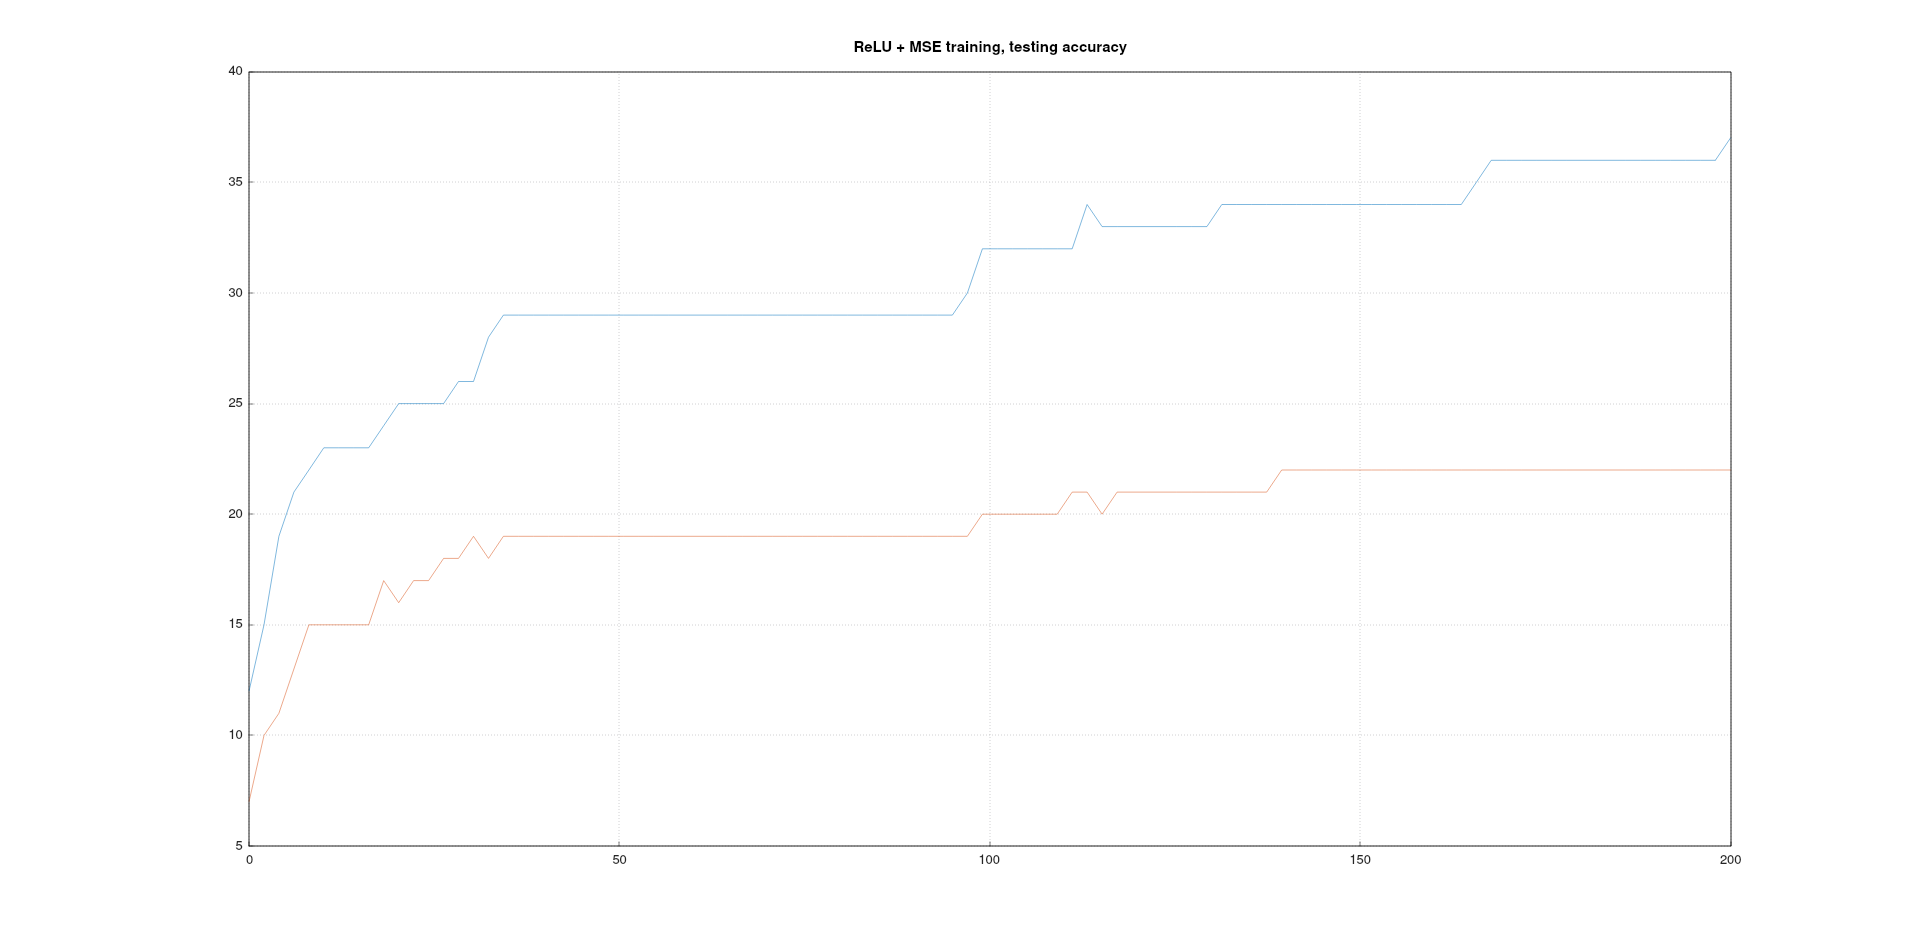
\includegraphics[width=\textwidth]{images/relu_mse_accuracy.png}
  \caption{}
  \label{fig:relu_mse_accuracy}
\end{figure}

\subsection{Функция сигмоиды}

Коэффициент обучения --- $5$.

На рисунке \ref{fig:sigmoid_mse_cost} изображено изменение функции ошибки за период обучения персептрона. В результате, ошибка на данных
для обучения составляет $0.028494$, ошибка на тестовых данных --- $0.03111$.

\begin{figure}[!htb]
  \centering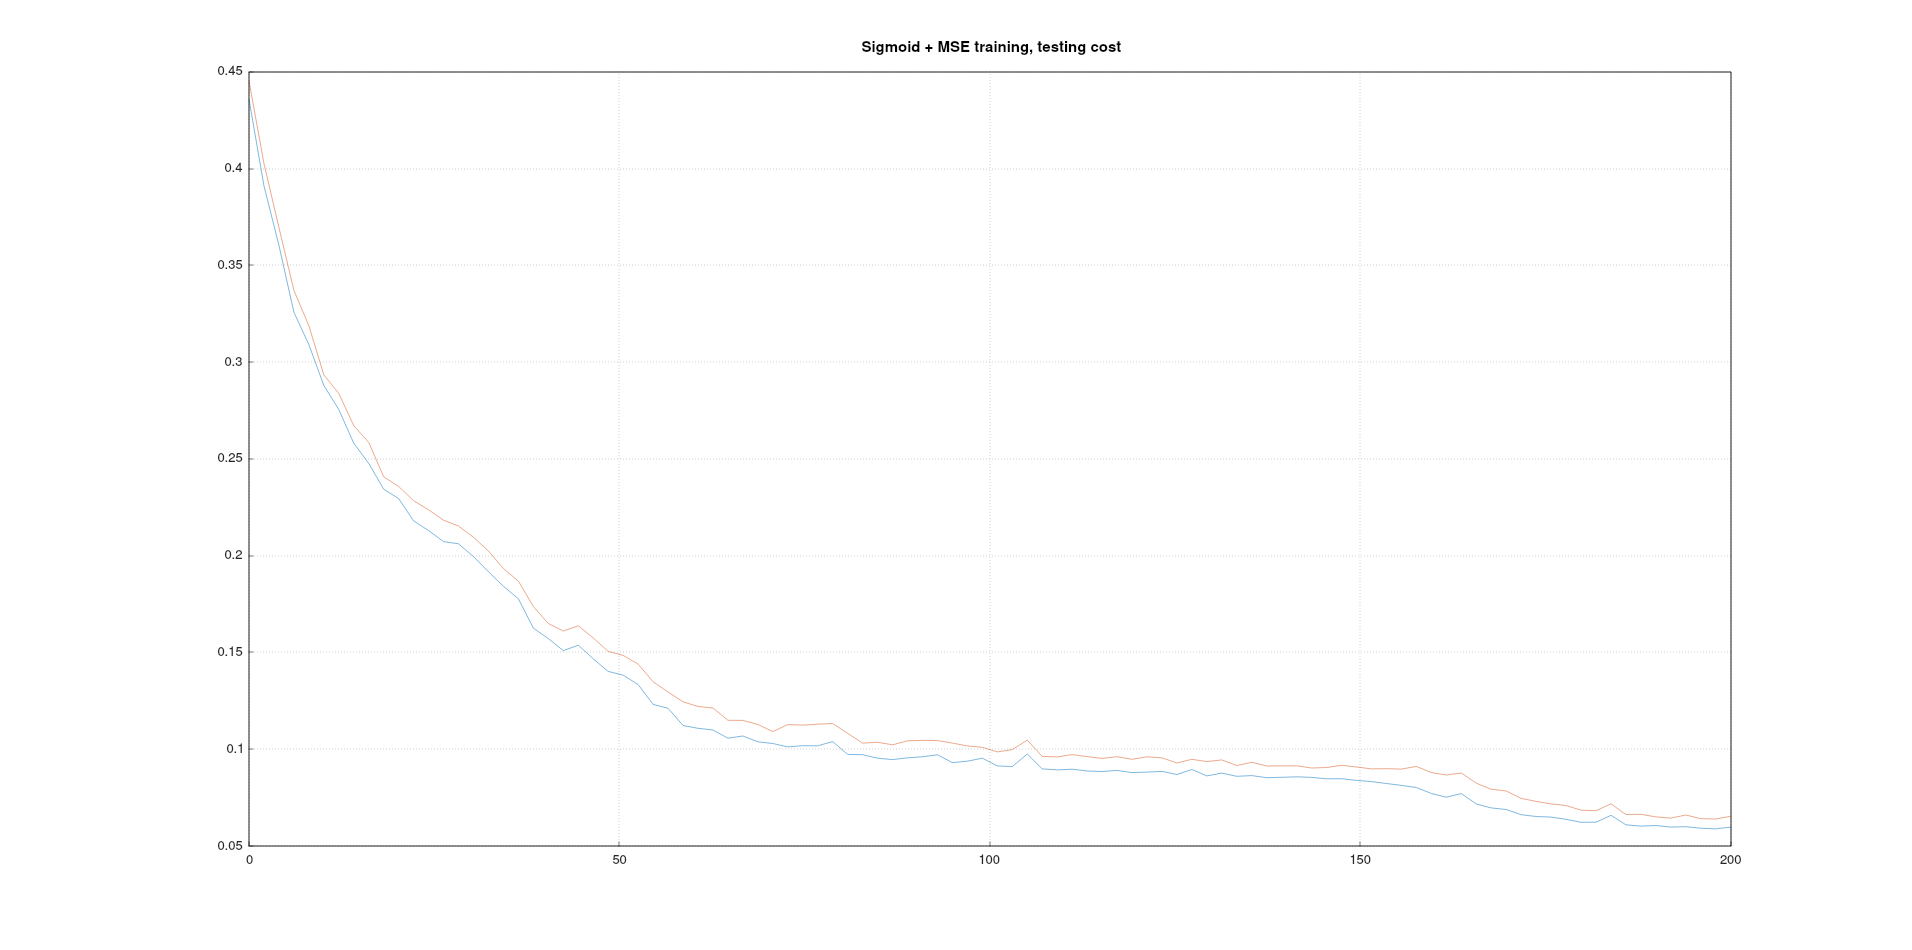
\includegraphics[width=\textwidth]{images/sigmoid_mse_cost.png}
  \caption{}
  \label{fig:sigmoid_mse_cost}
\end{figure}

На рисунке \ref{fig:sigmoid_mse_accuracy} изображено изменение точности за период обучения персептрона.
В результате, точность на данных для обучения составляет $\frac{152}{160}$, на тестовых данных --- $\frac{95}{100}$.

\begin{figure}[!htb]
  \centering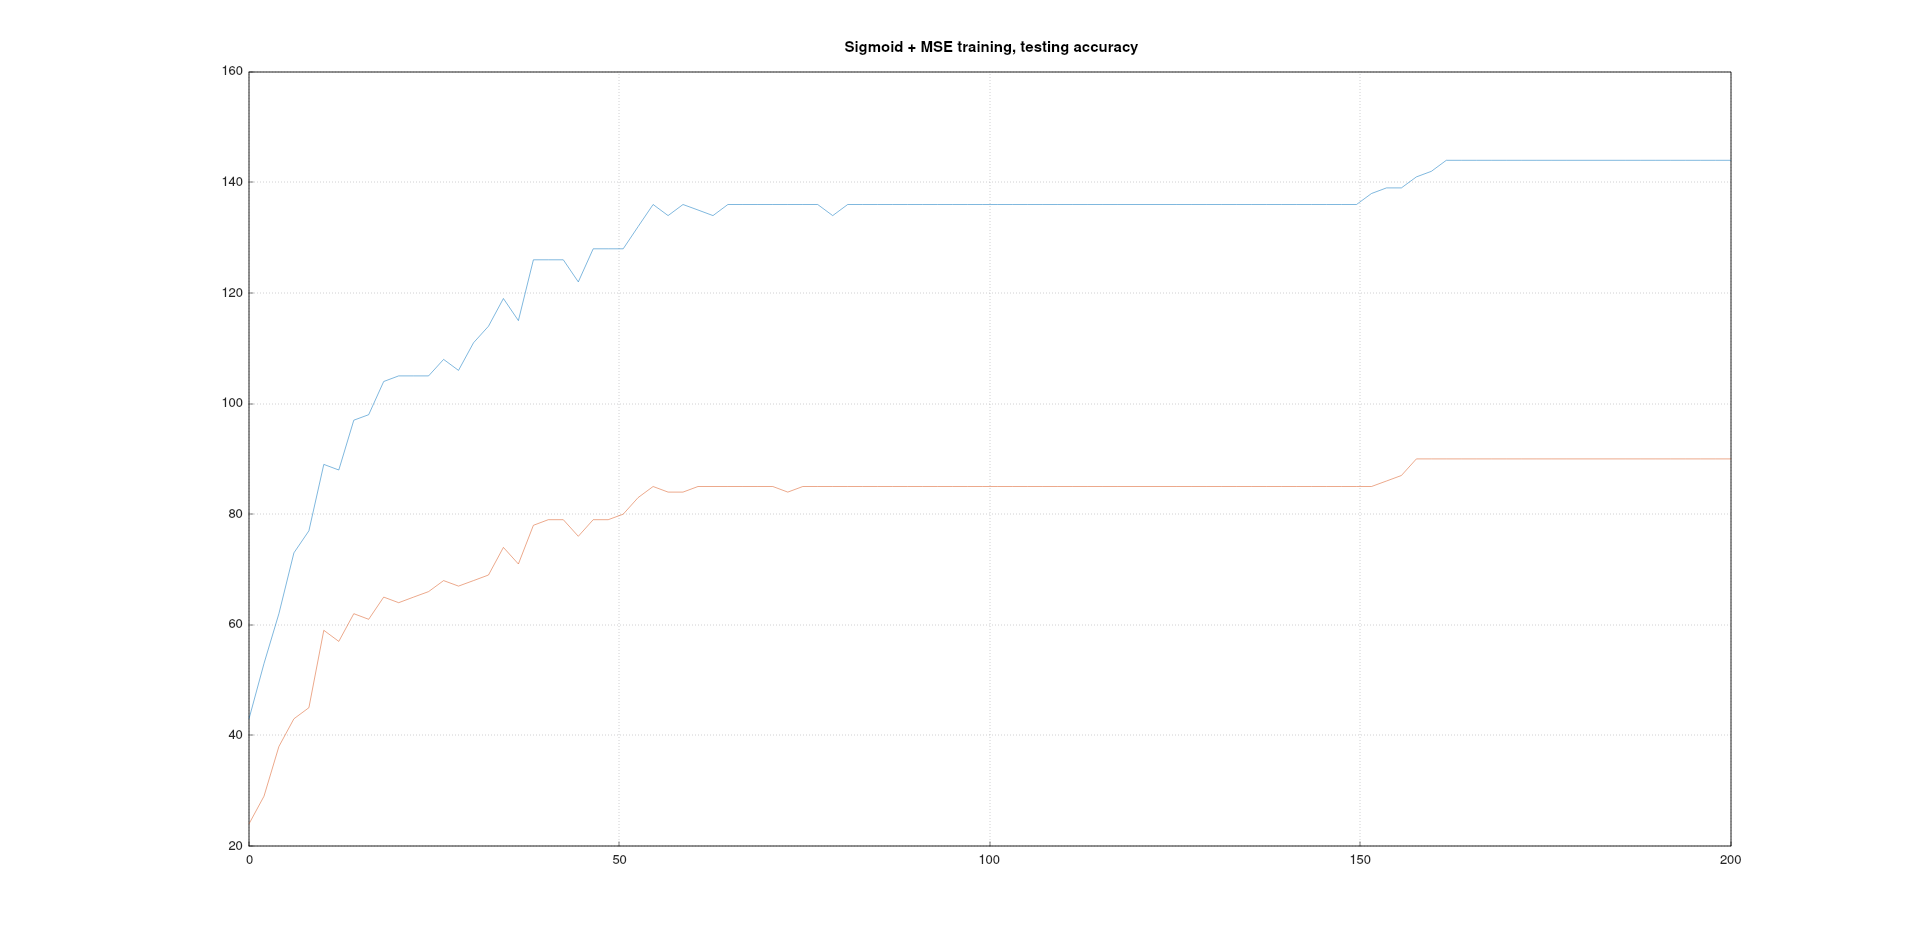
\includegraphics[width=\textwidth]{images/sigmoid_mse_accuracy.png}
  \caption{}
  \label{fig:sigmoid_mse_accuracy}
\end{figure}

\subsection{Функция гиперболического тангенса}

Коэффициент обучения --- $0.5$.

На рисунке \ref{fig:tanh_mse_cost} изображено изменение функции ошибки за период обучения персептрона.
В результате, ошибка на данных для обучения составляет $0.70365$, ошибка на тестовых данных --- $0.710095$.

\begin{figure}[!htb]
  \centering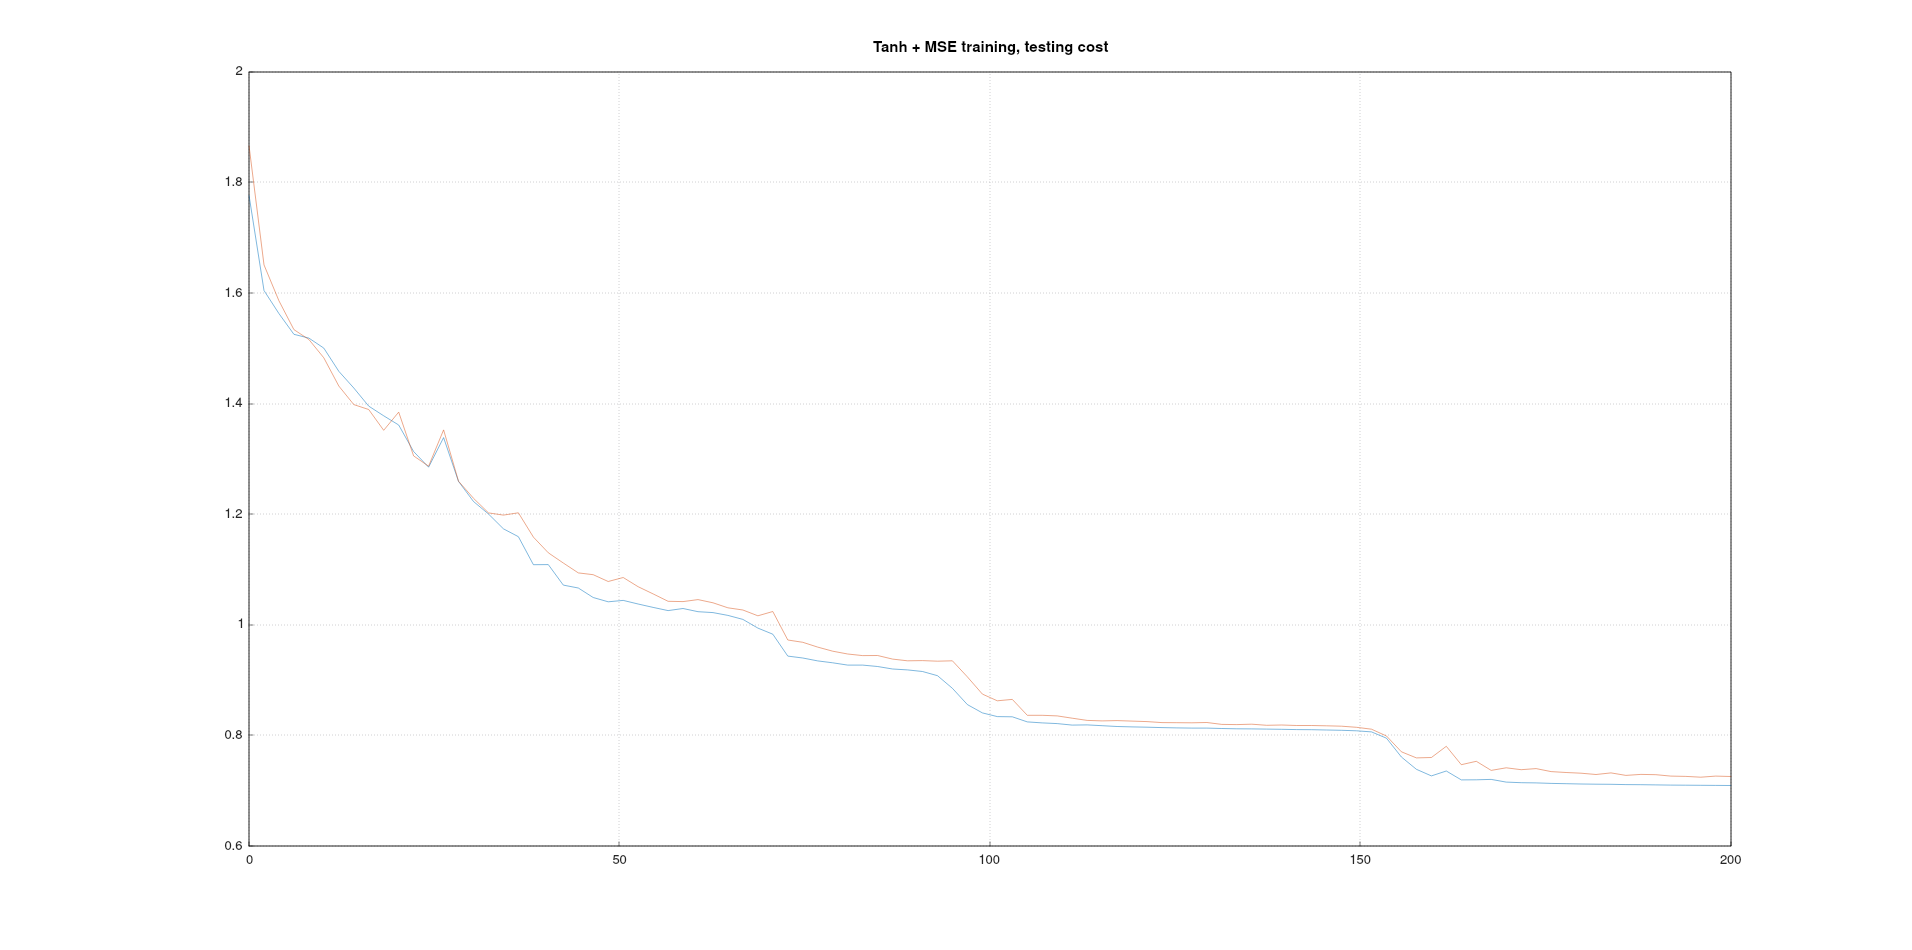
\includegraphics[width=\textwidth]{images/tanh_mse_cost.png}
  \caption{}
  \label{fig:tanh_mse_cost}
\end{figure}

На рисунке \ref{fig:tanh_mse_accuracy} изображено изменение точности за период обучения персептрона.
В результате, точность на данных для обучения составляет $\frac{104}{160}$, на тестовых данных --- $\frac{65}{100}$.

\begin{figure}[!htb]
  \centering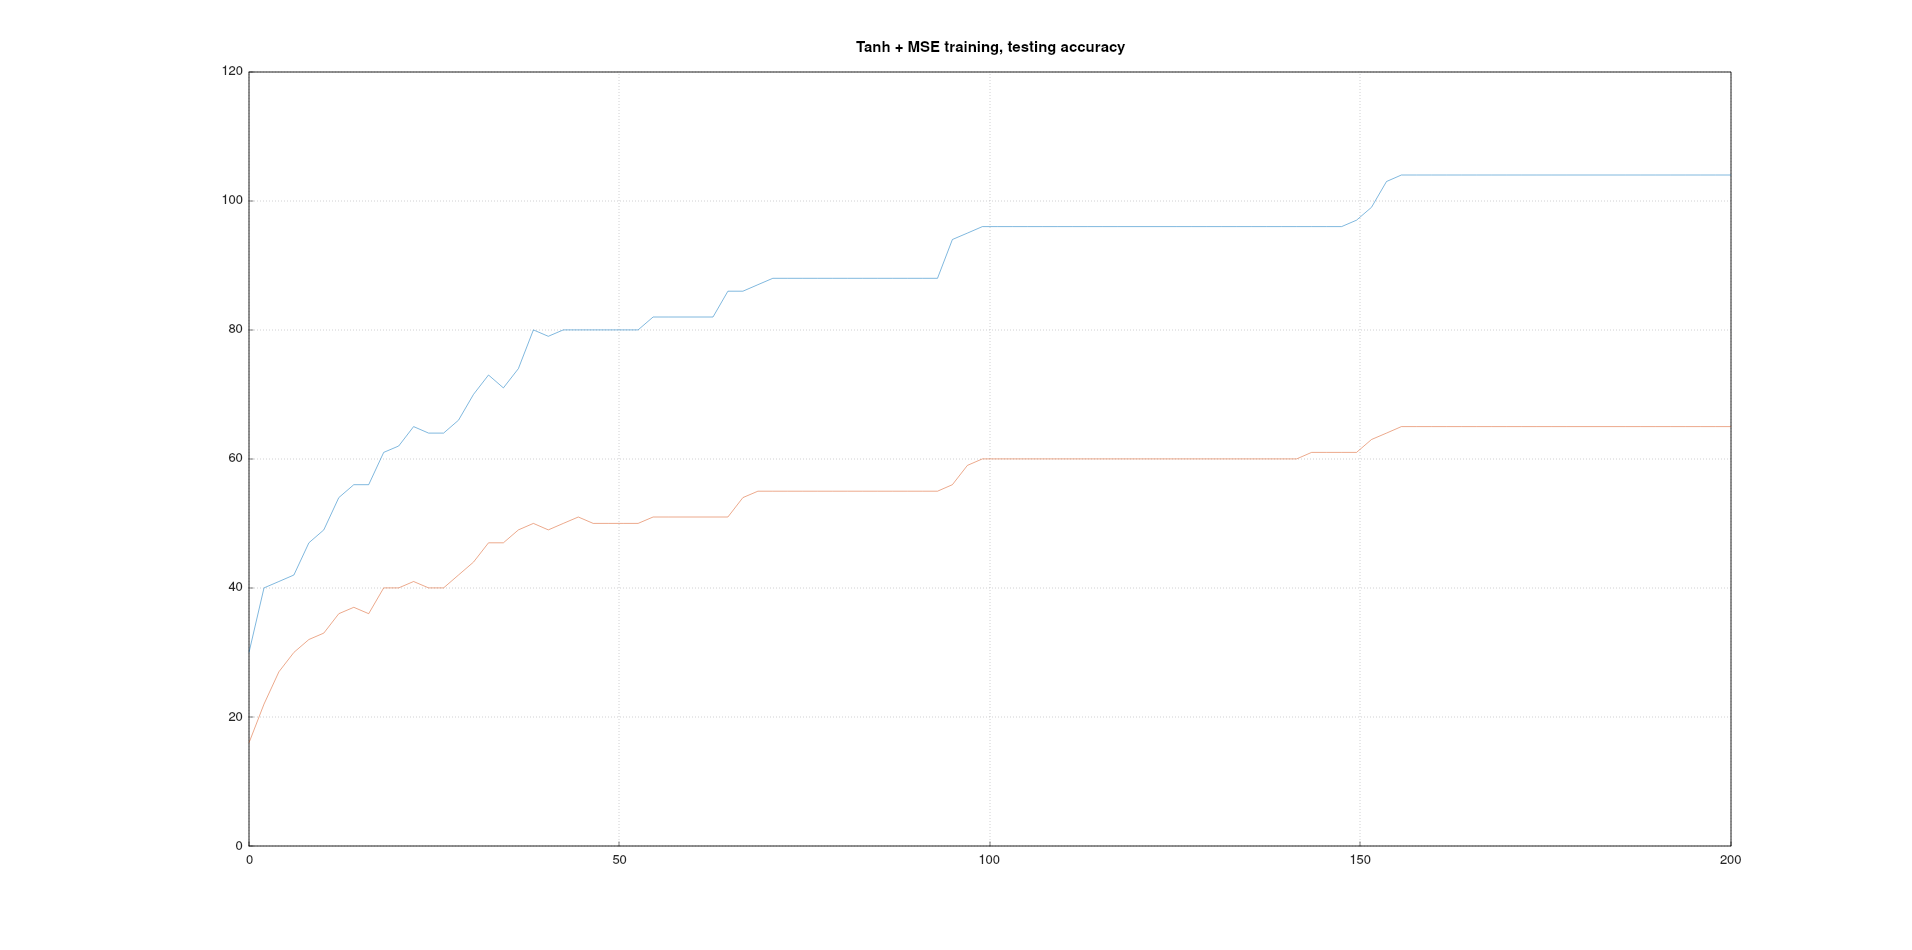
\includegraphics[width=\textwidth]{images/tanh_mse_accuracy.png}
  \caption{}
  \label{fig:tanh_mse_accuracy}
\end{figure}

\subsection{Функция Softmax}

Коэффициент обучения --- $10$.

Дополнительно произведено обучение персептрона с функцией активации Softmax и кросс-энтропией в качестве функции ошибки.

На рисунке \ref{fig:softmax_cross_entropy_cost} изображено изменение функции ошибки за период обучения персептрона.
В результате, ошибка на данных для обучения составляет $0.000196681$, ошибка на тестовых данных --- $0.0104362$.

\begin{figure}[!htb]
  \centering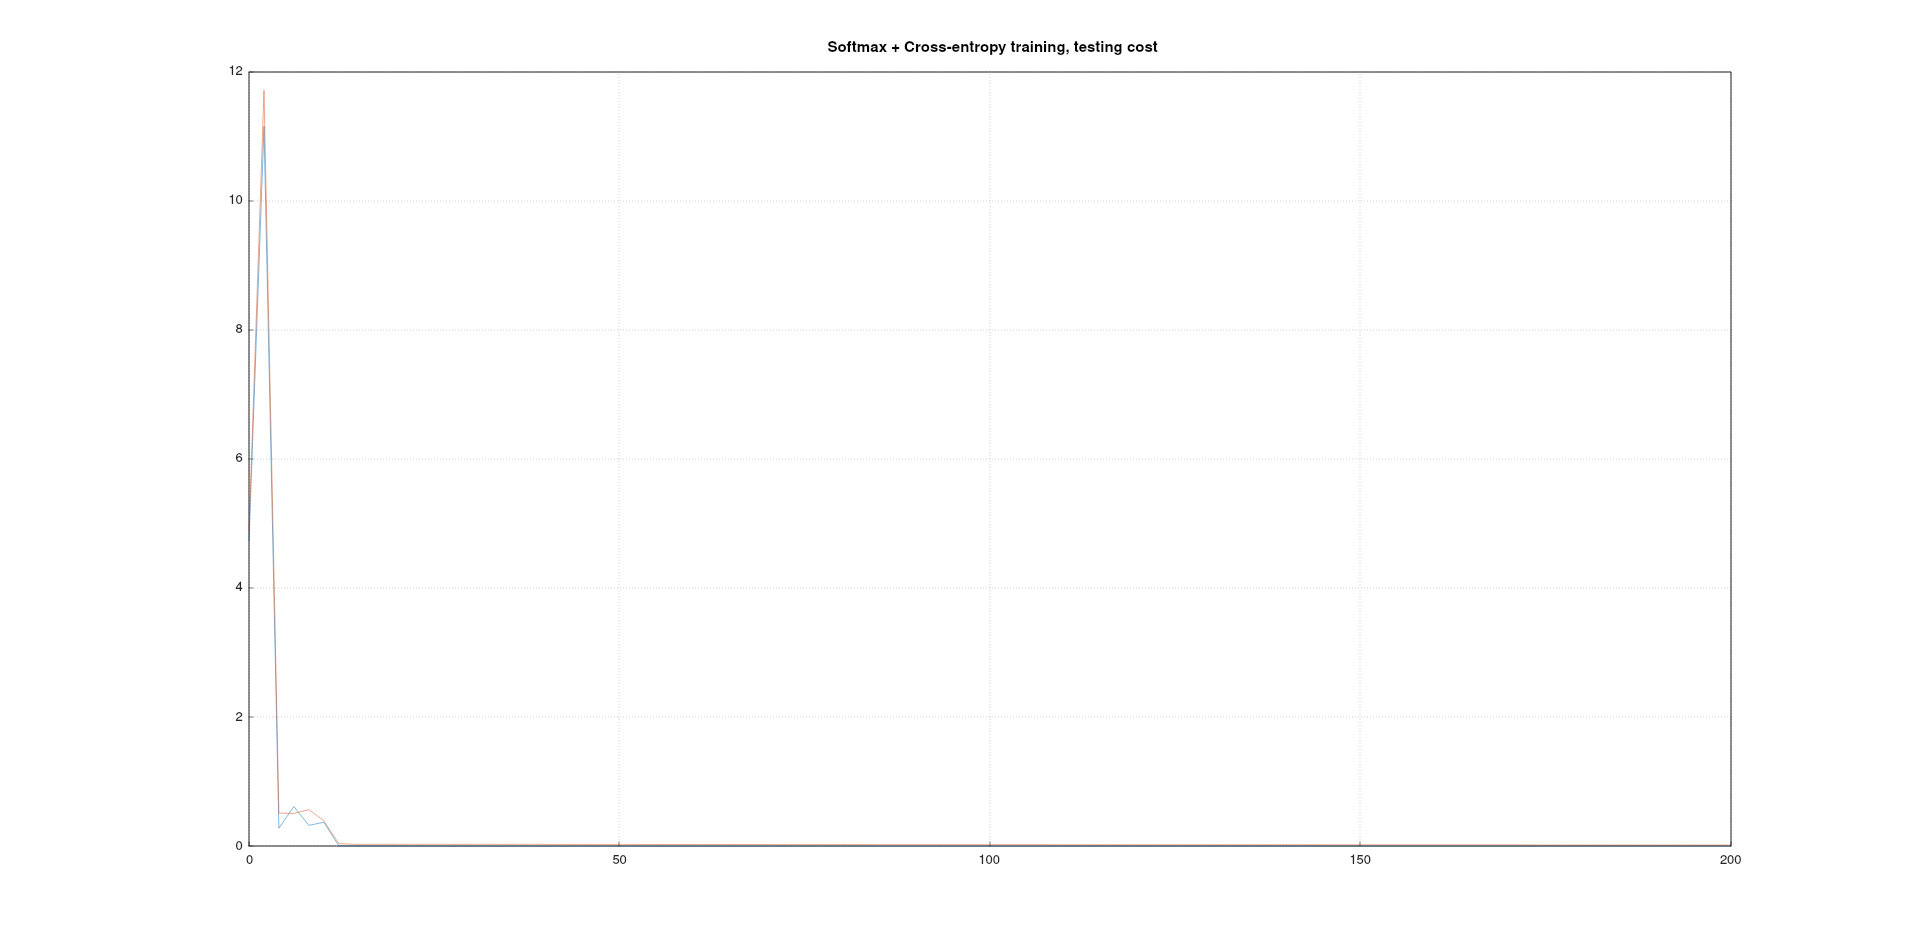
\includegraphics[width=\textwidth]{images/softmax_cross_entropy_cost.png}
  \caption{}
  \label{fig:softmax_cross_entropy_cost}
\end{figure}

На рисунке \ref{fig:softmax_cross_entropy_accuracy} изображено изменение точности за период обучения персептрона.
В результате, точность на данных для обучения составляет $\frac{160}{160}$, на тестовых данных --- $\frac{100}{100}$.

\begin{figure}[!htb]
  \centering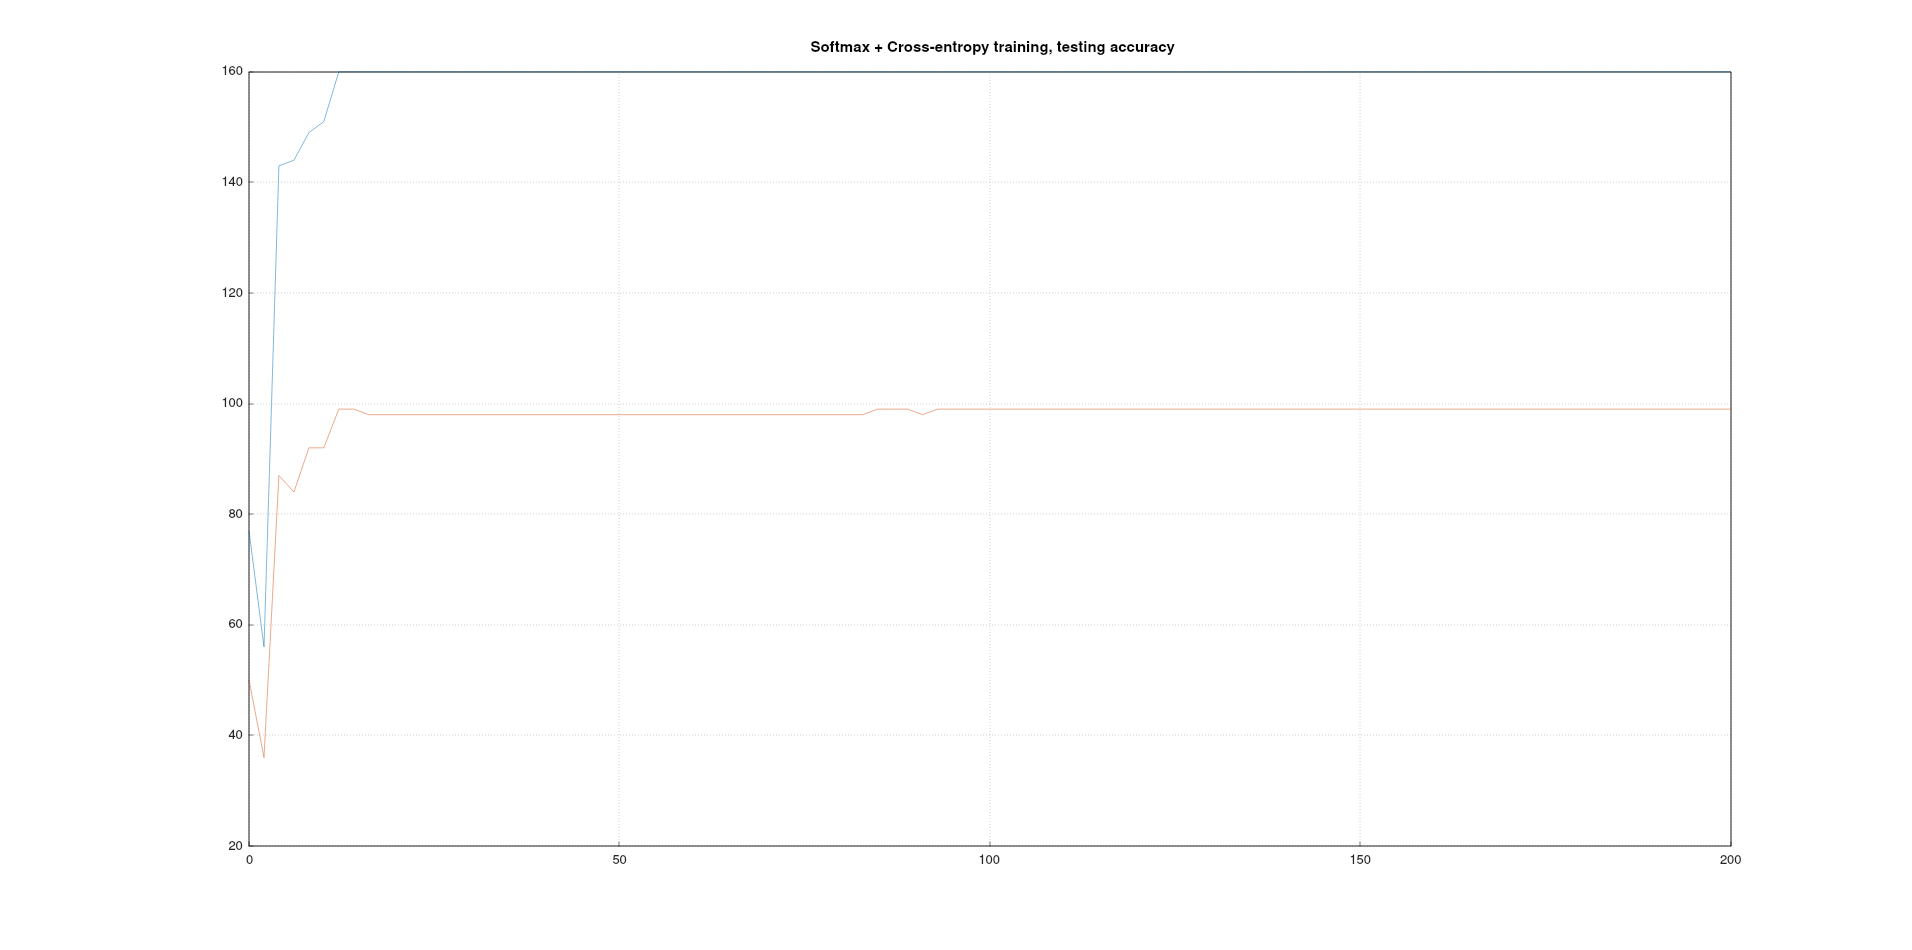
\includegraphics[width=\textwidth]{images/softmax_cross_entropy_accuracy.png}
  \caption{}
  \label{fig:softmax_cross_entropy_accuracy}
\end{figure}

\section{Вывод}

В результате выполнения домашней работы мне удалось реализовать каркас многослойного персептрона с обучением методом стохастического градиентного
спуска и вычислением градиентов методом обратного распространения ошибки. Персептрон может иметь произвольное число скрытых слоёв и быть параметризован
различными функциями активации и ошибки. Полученный каркас может быть расширен и совершенствован (например, с добавлением техник регуляризации).

По результатам экспериментов для однослойного персептрона видно:
\begin{itemize}
  \item линейная функция активации непригодна для использования на выходном слое в рамках поставленной задачи классификации;
  \item функция ReLU на выходном слое также показывает низкий результат точности в $25\%$ (на тестовых данных) --- функция предназначена для
    использования в \textit{скрытых} слоях персептрона;
  \item сигмоида показывает хороший результат точности в $95\%$.
  \item гиперболический тангенс показывает посредственный результат точности в $\%65$;
  \item дополнительно протестированные Softmax + кросс-энтропия показывают отличный результат точности $100\%$, который достигается всего за 10 эпох
    обучения.
\end{itemize}

Мне показался удивительным разрыв в точности между персептронами c сигмоидой и гиперболическим тангенсом. Вероятно, с лучшей настройкой гиперпараметров
результат для гиперболического тангенса может быть улучшен.

\end{document}
